\setAuthor{Valter Kiisk}
\setRound{lahtine}
\setYear{2023}
\setNumber{G 3}
\setDifficulty{3}
\setTopic{TODO}

\prob{Kummipael}
\begin{wrapfigure}[8]{r}{0.5\linewidth}
    %\vspace{-10pt}
    \begin{center}
        \vspace{5pt}
        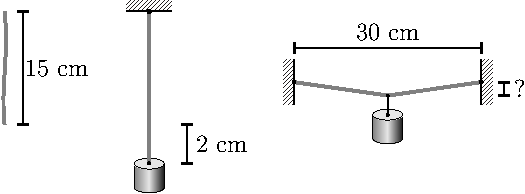
\includegraphics[width=\linewidth]{2023-lahg-03-yl.pdf}
    \end{center}
\end{wrapfigure}


Kummipaela pikkus vabas olekus on $L=\SI{15}{cm}$. Kui kummipaela külge riputati tundmatu massiga koormis, siis kummipaela pikkus kasvas $\Delta L=\SI{2}{cm}$ võrra (vt joonis). Seejärel kummipael fikseeriti otstest kahe samal kõrgusel paikneva punkti vahele, mille vahekaugus oli $2L$ (st pael venitati $L$ võrra pikemaks). Sama koormis riputati nüüd kummipaela keskpunkti. Hinnake, kui suur on selle punkti läbivajumine. Võib eeldada, et kummipaelas tekkiv elastsusjõud on võrdeline pikenemisega ja kummipaela enda mass on tühine.\\ \emph{Märkus:} Väikeste nurkade $x$ korral võib kasutada lähendust $\sin{x} \approx \tan{x} \approx x$ (nurk $x$ on radiaanides).










\hint

\solu
Esimese katse jaoks saame jõudude tasakaalutingimuse $k\Delta L=mg$, kus $k$ on kummipaela jäikustegur ja $m$ on koormise mass (mõlemad tundmatud). Siit saame avaldada suhte $mg/k=\Delta L$. Teises katses on kummipael juba algselt tugevasti deformeeritud olekus, kus tõmbejõud kummipaelas on $kL$ (sest pikkuse muut on $L$). Eeldame, et seetõttu läbivajumine $x\ll L$. Sel juhul, ühelt poolt, läbivajumisest tingitud kummipaela pikenemine on tühine ja seeläbi ka pinge paelas jääb peaaegu muutumatuks. Teiselt poolt, kummipael moodustab horisontaalsihiga nurga $\varphi\approx x/L$. Piki kummipaela suunatud jõu $kL$ projektsioon vertikaalsihile on siis ilmselt $kL\sin\varphi\approx kL\varphi\approx kx$. Kuivõrd kuumipaelal on nüüd kaks poolt, mis mõlemad ühtviisi panustavad koormise $mg$ tasakaalustamisse, siis $2kx=mg$, millest
\[
x =\frac{mg}{2k} =\frac{\Delta L}{2} = \SI{1}{cm}.
\]
\probend